\documentclass[a4paper,12pt]{report}
\usepackage[slovak,english]{babel}
\usepackage[T1,IL2]{fontenc}             
\usepackage[utf8]{inputenc}    
\usepackage{amsmath}
\usepackage{amssymb,amsfonts,amscd}
\usepackage{array,hhline}
\usepackage{makeidx}
\usepackage{fancyhdr}
\usepackage{graphicx}
\usepackage{listings}
\usepackage{eurosym}
\usepackage{url,mathptmx} 
\usepackage[pdftex,unicode,bookmarks=false]{hyperref}
\usepackage{comment}
\renewcommand{\baselinestretch}{1.5} 
\addtolength{\oddsidemargin}{-.5cm}
\addtolength{\evensidemargin}{-2.9cm}   
\addtolength{\topmargin}{0cm}
\addtolength{\textheight}{0pt}
\addtolength{\textwidth}{2.cm}
\addtolength{\textheight}{2.cm}
\newlength{\verbcorr}
\setlength{\verbcorr}{0ex}
\usepackage{acronym}
%pre nastavenie formatovania kodu TODO vylepsit
\lstset{%
	language={Java},
	breaklines=true,
	breakindent=0pt,
	tabsize=2,
	showstringspaces=true
}

\usepackage{lmodern}%INE pismo
%\usepackage{type1ec}
\usepackage{float}%H pri tabulkach
\usepackage{pdfpages}

\begin{document}


\selectlanguage{slovak}
\pagestyle{empty}
\pagenumbering{arabic}
\begin{titlepage}
\phantom.

\bigskip

\begin{center}
{\sc\LARGE Žilinská Univerzita v Žiline}
\medskip

{\sc\Large Fakulta riadenia a informatiky}

\vfill\vfill\vfill\vfill

{\sc\LARGE Diplomová práca}

\medskip

{\large Študijný odbor: {\bf Informačné systémy - Spracovanie dát}}
\end{center}


\vfill\vfill\vfill\vfill


\phantom.\hfill

\begin{center}
{\large\bf Oľga Chovancová}

\medskip

{\large\bf Nástroj pre fuzzifikáciu numerických hodnôt}

\medskip

Vedúci: {\bf Ing. Miroslav Kvaššay, PhD.}
\medskip
 
\hfill
Reg.č. 6/2016
\hfill
Máj 2017
\hfill\phantom.
\end{center}

\hspace{1.7cm}\phantom.

\vspace{2.9cm}

\phantom.
\end{titlepage}
%%%%%%%%%%%%%%%%%%%%%%%%%%%%%%%%%%%%%%%%%%%%%%%%%%%%%%%%%%%%%%%%%%%%%%%%%%%%%%%%%%%%%%%%%%%%%%%%%%%%%%%%%%%%%%%%%%%%%%%%%%%%%%%%%%%%%%%%%%%%%%%%%%%%%%%%%%%%%%%%%%%%%%%%%%%%%%%%%%%%%%%%%%%%%%%%%%%%%%%%%%%%%%%%%%%%%%%%%%%%%%%%%%%%%%%%%%%%%%%%%%%%%%%%%%%%%%%%

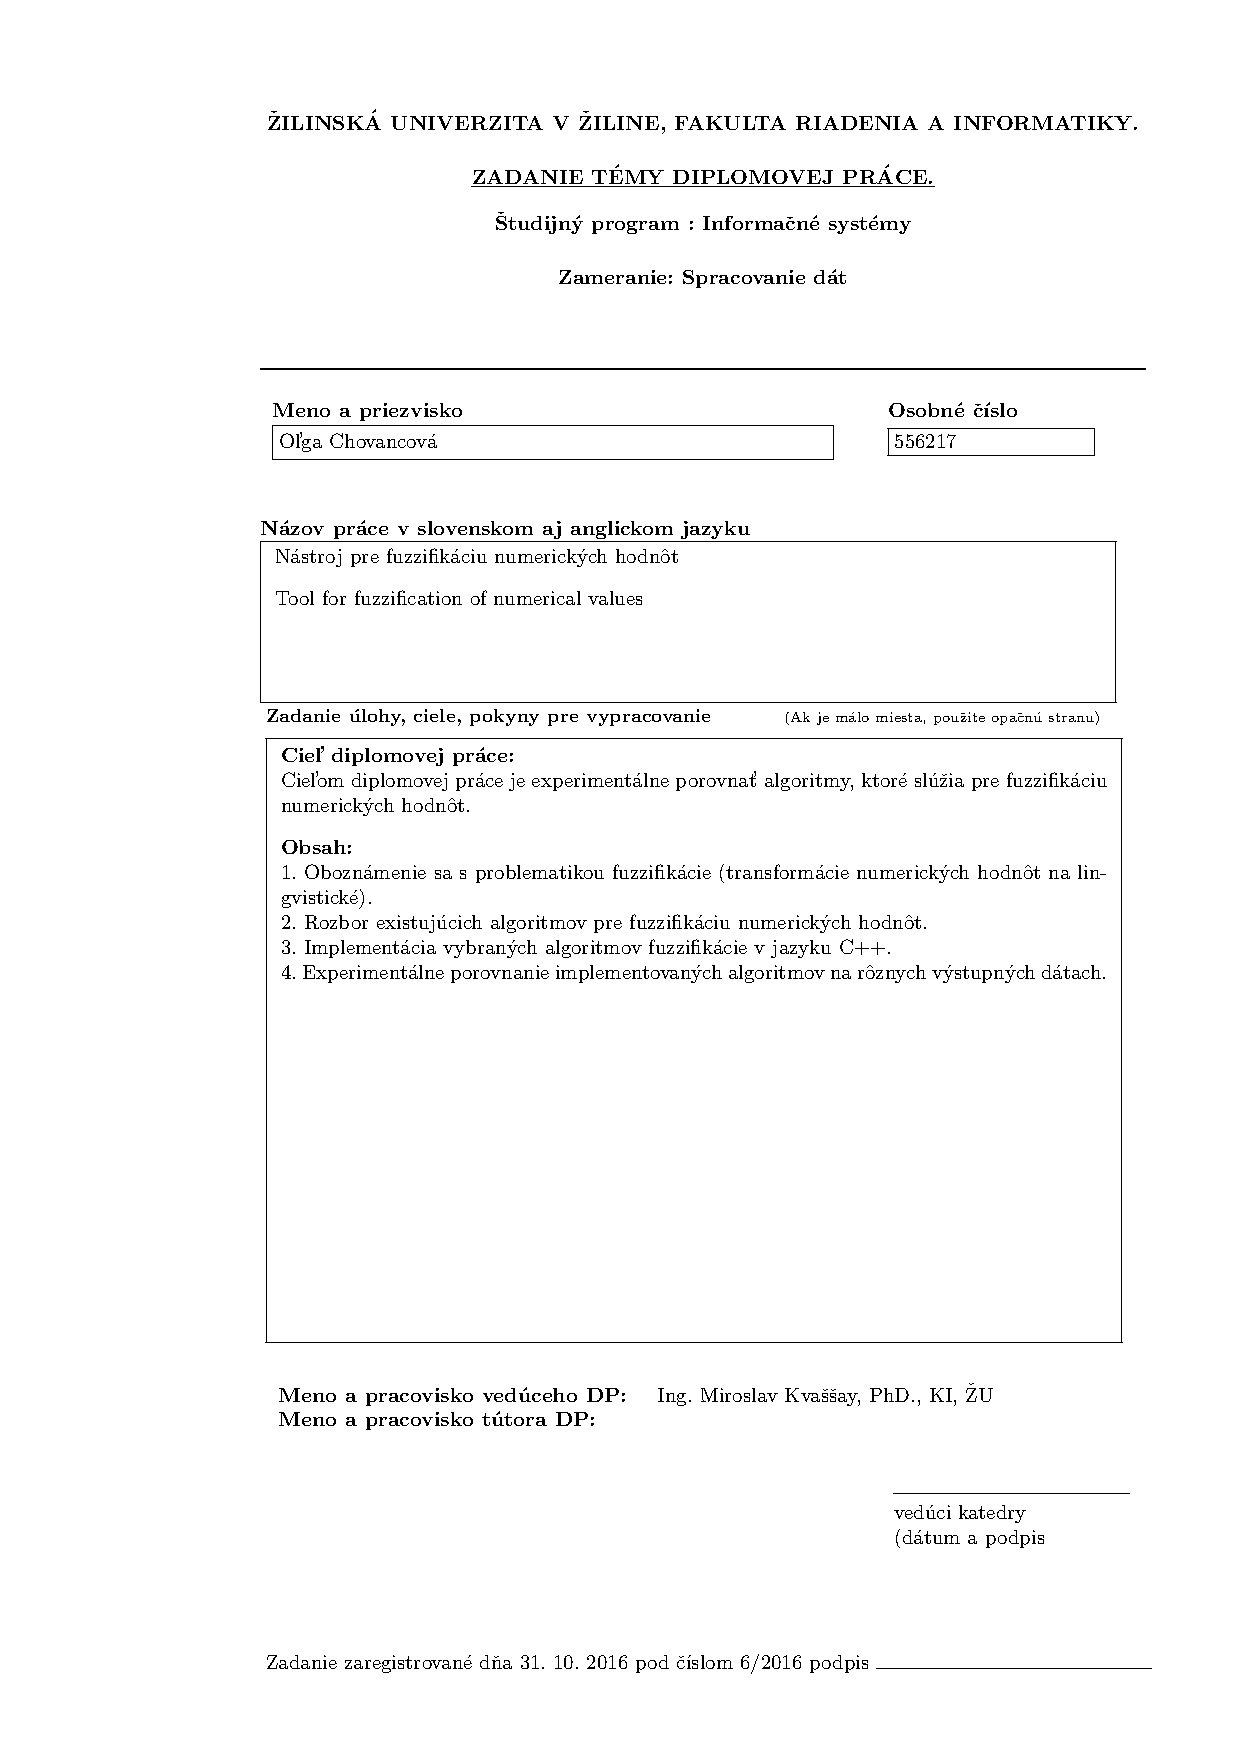
\includepdf{zadanie.pdf}

\newpage

\centerline{\bf Čestné prehlásenie}

\vspace{2em}

\noindent
Prehlasujem, že som diplomovú prácu \textit{Nástoj pre fuzzifikáciu numerických hodnôt} vypracovala samostatne pod vedením ... , a uviedla v nej všetky použité literárne a iné odborné zdroje v súlade s právnymi predpismi, vnútornými predpismi Žilinskej univerzity a vnútornými aktmi riadenia Žilinskej univerzity a Fakulty riadenia a informatiky.

\vspace{2em}

\noindent
V~Žiline, dňa XX.05.2017
\hfill
Oľga Chovancová

\newpage


\newpage

\centerline{\bf Poďakovanie}
\vspace{2em}
\noindent
%Prehlasujem, že som túto prácu napísala samostatne a že som uviedola
%všetky použité pramene a literatúru, z~ktorých som čerpala. 

\bigskip

Na tomto mieste by som chcela poďakovať vedúcemu diplomovej práce....  za cenné pripomienky a odborné rady, ktorými prispel k vypracovaniu tejto diplomovej práce. Taktiež ďakujem môjmu ... . Zároveň ďakujem mojej rodine a priateľom za ich nekonečnú podporu a trpezlivosť. 

\vspace{2em}

\noindent
V~Žiline, dňa XX.05.2017
\hfill
Oľga Chovancová	
%--------------------------------------------------------------------------------------
%%% slovensky abstrakt

\begin{abstract}

\noindent
{\sc Chovancová Oľga:} {\em Nástroj pre fuzzifikáciu numerických hodnôt}
[Diplomová práca] 

\noindent
Žilinská Univerzita v~Žiline,  
Fakulta riadenia a informatiky,  
Katedra informatiky.

\noindent  
Vedúci: Ing. Miroslav Kvaššay, PhD.
 
\noindent  
Stupeň odbornej kvalifikácie:
Inžinier** Informatiky
%Inžinier v študijnom odbore Telekomunikačné siete, na Elektrotechnickej fakulte na Žilinskej univerzite v Žiline. 


\bigskip
Cieľom diplomovej práce je experimentálne porovnať algoritmy, ktoré slúžia pre fuzzifikáciu numerických hodnôt. 

 
1. Oboznámenie sa s problematikou fuzzifikácie (transformácie numerických hodnôt na lingvistické).
2. Rozbor existujúcich algoritmov pre fuzzifikáciu numerických hodnôt.
3. Implementácia vybraných algoritmov fuzzifikácie v jazyku C++.
4. Experimentálne porovnanie implementovaných algoritmov na rôznych výstupných dátach.

\noindent
\bigskip
Kľúčové slová: fuzzy, TODO

\end{abstract}


%--------------------------------------------------------------------------------------
%%% anglicky abstrakt


\selectlanguage{english}
\begin{abstract}

\noindent
{\sc Chovancová Oľga:} {\em Tool for fuzzification of numerical values}
[Diploma thesis] 

\noindent
University of Žilina,  
Faculty of Management Science and Informatics, 
Department of Informatics 
 
\noindent
Tutor:  Ing. Miroslav Kvaššay, PhD.

 
\noindent
Qualification level: 
Masters of Informatics
 

\noindent


\bigskip

The aim of the thesis is to compare experimental algorithms that are used for Fuzzification numerical values.
\\
TODO
\\
1. This introduction to the Fuzzification (numeric values to transform linguistic).
2. Analysis of the existing algorithms for fuzzification numerical values.
3. Implementation of selected algorithms Fuzzification in C ++.
4. Experimental comparison algorithms implemented on different output data.
\noindent
\bigskip
Key words: fuzzy, entropy, TODO

\end{abstract}
\selectlanguage{slovak}	

\pagestyle{empty}
\pagenumbering{arabic} 
\pagestyle{plain}	%F
\setcounter{page}{6} %F


{\setlength{\parskip}{1pt plus 1pt}

\markboth{}{}
\tableofcontents

\newpage
%
\vspace{0pt plus 2cm}
%
\listoffigures
%
\vspace{0pt plus 2cm}
%
\listoftables
\vspace{0pt plus 2cm}

\chapter*{Zoznam skratiek}
\begin{acronym}
\acro{FEBFC}{Fuzzy entropy-based fuzzy classifier}



%diskretizacne metody
\acro{EqualWidth}{Equal Width Discretizer}
\acro{EqualFrequency}{Equal Frequency Discretizer } 
\acro{ID3}{Iterative Dichotomizer 3 Discretizer } 
\acro{MDLP}{Minimum Description Length Principe} 
\acro{CADD}{Class-Attribute Dependent Discretizer } 
\acro{StatDisc}{Class-driven Statistical Discretizer} 
\acro{BRDisc }{Boolean Reasoning Discretizer } 
\acro{MDL-Disc }{Minimum Description Length Discretizer } 
\acro{Bayesian }{Bayesian Discretizer } 
\acro{CAIM }{Class-Attribute Interdependence Maximization } 
\acro{WEDA }{Wrapper Estimation of Distribution Algorithm } 
\acro{EBDA }{Effective Botton-up Discretizer } 
%\acro{ }{ } 

 
\end{acronym}

%pridat typy licencie..
}
\markboth{}{}
\clearpage
\clearpage
\clearpage
\setcounter{page}{14} %F

\chapter*{Úvod}
\addcontentsline{toc}{chapter}{Úvod}

Cieľom diplomovej práce je experimentálne porovnať algoritmy, ktoré slúžia pre fuzzifikáciu numerických hodnôt.

Náplňou prvej časti práce je oboznámenie sa s problematikou fuzzifikácie.  

Ďalšia časť sa zaoberá rozborom existujúcich algoritmov pre fuzzifikáciu numerických hodnôt na lingvistické. 

Ďalšia kapitola popisuje spôsob implementácie vybraných algoritmov fuzzifikácie v jazyku C++. 

Posledná časť práce experimentálne porovnáva dané implementácie na rôznych výstupných dátach. 


\chapter{Analýza súčasného stavu}



\chapter{Cieľ práce}
Cieľom diplomovej práce je experimentálne porovnať algoritmy, ktoré slúžia pre fuzzifikáciu numerických hodnôt.

\section*{Postup práce}
 
\begin{enumerate}
\item Oboznámenie sa s problematikou fuzzifikácie (transformácie numerických hodnôt na lingvistické).
\item Rozbor existujúcich algoritmov pre fuzzifikáciu numerických hodnôt.
\item  Implementácia vybraných algoritmov fuzzifikácie v jazyku C++.
\item  Experimentálne porovnanie implementovaných algoritmov na rôznych výstupných dátach.
\end{enumerate}

















	
\chapter{Teoretické východiská práce} 

\section{Fuzzy dáta a expertné odhady}
%todo pridat do zoznamu zdrojov a potom to tuto v tejto kapitole citovať
%z knihy Projektovanie systémov pre podporu rozhodovania na základe neurčitých dát, Vitaly Levasheko, Elena Zaitseva, Štefan Kovalík, Vydala Žilinská univerzita v Žiline/Edis-vydavateľstvo ŽU, 2013, ISBN 978-80-554-0680-0
%5 strana
Metódy a algoritmy využívané v súčasných systémoch pre podporu rozhodovania by mali brať do úvahy možnú nestochastickú neurčitosť vstupných dát, spôsobenú nedostatočnou presnosťou merania. Jeden z prístupov, ktorý berie do úvahy neurčitosť, je vyjadrenie vstupných hodnôt pomocou neurčitých fuzzy dát alebo pomocou viachodnotových dát. 
Matematickým aparátom spracovania neurčitých dát a viachodnotových dát je fuzzy logika a viac hodnotová logika. \cite{levashenkoProj}
\paragraph{}
%6 strana
Neurčité dáta sa reprezentujú pomocou lingvistických premenných, ktorých hodnoty patria do konečnej množiny. \cite{levashenkoProj}
%9 strana
Lingvistické premenné sa javia ako jeden z často používaných spôsobov vyjadrenia hodnôt, opisovaných kvantitatívnymi 
%10 strana
alebo kvalitatívnymi veličinami. Kvalitatívne veličiny sa v mnohých prípadoch javia ako výsledok formalizácie expertných odhadov. \cite{levashenkoProj}
%10 strana = kapitola 1.1 kapitola o fuzzy dáta a expertné odhady. 
Každý objekt alebo proces sa opisuje skupinou ukazovateľov. V modeloch pre podporu rozhodovania sa využívajú ukazovatele, ktoré nadobúdajú hodnoty z množiny reálnych čísel. 
Dôvody, ktoré sťažujú použitie reálnych čísiel sú nasledovné: \cite{levashenkoProj}
%todo treba preštylizovat todo 
\begin{enumerate}
	\item Zložitosť presného merania hodnôt ukazovateľa. 
	\item Nie sú algoritmy a metódy výpočtu presných hodnôt ukazovateľa. 
	\item Zložitosť dostupnosti nameraných dát, súvisiaca s radom objektívnych a subjektívnych faktorov. 
	\item Absencia nevyhnutnosti poznať presné hodnoty. 
	\item Relatívne vysoké náklady na zmeranie presných hodnôt ukazovateľov. 
\end{enumerate}
%todo doslovne citovanie. treba prestylizovat  
Reálne hodnoty jednotlivých ukazovateľov bez prihliadnutia na iné ukazovatele jednej strane nesú pre výber rozhodnutia zbytočne podrobnú informáciu o tomto ukazovateli, na druhej strane nemôžu byť základom pre výber rozhodnutia. \cite{levashenkoProj}
%11 strana
Z toho vyplýva, že sa ukazuje ako užitočné využiť približné, neurčité fuzzy hodnoty vstupných dát. 
Použitie podobných fuzzy hodnôt umožňuje zaviesť do výskumu kvalitatívne opisy. Vo výsledku sa berie do úvahy neurčitosť úlohy rozhodovania, zabezpečuje sa adekvátny opis všetkých faktorov, ktoré majú vzťah danej, ale nie je možné zabezpečiť ich presný kvantitatívny opis. 
\paragraph*{}
Spracovanie neurčitej fuzzy informácie v rozhodovacích úlohách sa zabezpečuje aplikovaním lingvistického prístupu.\cite{levashenkoProj} %tuto este cituju Zadh1976, Lieb1993, Novak2005, Navara2007
Matematickým aparátom ich formalizácie je teória fuzzy množín. 


%todo prestylizovať todo
Lingvistický prístup pri konštrukcii modelov rozhodovania umožňuje\cite{levashenkoProj}: 
\begin{itemize}
	\item využiť na opis elementov úlohy rozhodovania subjektívne odhady expertov, vyjadrené pomocou neurčitých fuzzy pojmov, vzťahov a výrokov profesionálneho jazyka;
	\item formalizovať neurčité fuzzy opisy pomocou fuzzy množín a lingvistických premenných;
	\item spracovávať neurčité fuzzy opisy prostredníctvom matematického aparátu teórie fuzzy logiky. 
\end{itemize}

Základ tohto prístupu tvoria pojmy neurčitej fuzzy premennej a lingvistickej premennej. 
Medzi základné pojmy patrí definícia fuzzy množiny, fuzzy premennej, lingvistickej premennej, funkcie príslušnosti.\cite{levashenkoProj}

% tieto pojmy asi su aj v Zadeh1965, Zadeh1996 , citujem ich doslovne z knihy = Projektovanie systemov.. 
Nech $ X = \left\lbrace x \right\rbrace$ je množina prvkov x. 

\paragraph*{Definícia 1.} 
Fuzzy množina $A \subset X $ je predstavovaná množinou dvojíc $ \left\lbrace \left( x, \mu_A \left( x \right) \right) \right\rbrace  $, kde $ x \in X$ a $ \mu_A : X \longrightarrow \left\langle 0, 1\right\rangle $ je funkcia príslušnosti, ktorá predstavuje subjektívnu mieru príslušnosti elementu x k množine A. 
Veličina $\mu_A\left( x\right) $ nadobúda hodnoty od nuly, ktorá označuje absolútnu nepríslušnosť po hodnotu jedna, ktorá hovorí o absolútnej príslušnosti elementu x do fuzzy množiny A. \cite{levashenkoProj, Zadeh1965}
% toto bolo doslova asi citovane zo 
%Zadeh L., Fuzzy sets. Information and Control, vol.8, 1965, pp. 338-353. 

%12 strana knihy o projektovani systemov
Ak je fuzzy množina A definovaná na konečnej univerzálnej množine 
\\
 $X = \left\lbrace x_1, x_2, ... , x_i, ..., x_n\right\rbrace $, potom je vhodné označiť ju nasledovne
$$
A = \left\lbrace 
\left( x_1, \mu_A\left( x_1\right)  \right) , 
\left( x_2, \mu_A\left( x_2\right)  \right) , ... , 
\left( x_i, \mu_A\left( x_i\right)  \right) , ... , 
\left( x_n, \mu_A\left( x_n\right)  \right) 
 \right\rbrace , 
$$ 
kde $\left( x_i, \mu_A\left( x_i\right)  \right)$ - je dvojica tvorená elementov $x_i$ a jeho funkciou príslušnosti, nazývaná singleton. \cite{levashenkoProj}

%%tieto definicie su na strane 12, a su citovane z knihy, a aj Kaufmann1985, Klir1995, Navara2011

\paragraph*{Definícia 2. }
Fuzzy premenná je definovaná trojicou $\left( \alpha, X, A \right) $, kde 
$\alpha $ - je meno fuzzy premennej, 
 $X=\left\lbrace x \right\rbrace$ - je množina, tvoriaca definičný obor premennej x, 
 A - je fuzzy podmnožina fuzzy množiny X, pre každý prvok ktorej je definovaná funkcia $\mu_A\left( x\right)$, udávajúca stupeň príslušnosti daného elementu x do množiny A.  \cite{levashenkoProj}

\paragraph*{Definícia 3.}
Lingvistická premenná je definovaná päticou 
$
\left(
\beta, T, X, G, M
 \right) 
$, kde 
$\beta$ - je meno lingvistickej premennej; 
T - je množina jej hodnôt $\left( termov \right) $, z ktorých každá je fuzzy premennou na množine X;
G - je syntaktické pravidlo pre tvorbu nových mien hodnôt lingvistickej premennej $\beta$;
M - je sémantická procedúra, umožňujúca transformovať novú hodnotu premennej $\beta$, určenú procedúrou G, na fuzzy premennú, t.j. vytvoriť zodpovedajúcu fuzzy množinu. \cite{levashenkoProj}


\paragraph*{Definícia 4.}
Funkcia príslušnosti $\mu_A\left( x\right)$ kvantitatívne určuje príslušnosť elementov základnej množiny uvažovaného priestoru $x \in X$ k fuzzy množine A. Hodnota A tejto funkcie značí, že element nepatrí do fuzzy množiny, hodnota 1 opisuje úplne patriaci element. Hodnoty medzi 0 a 1 charakterizujú neurčito zaradené elementy. \cite{levashenkoProj, Kaufman1985, Klir1995, Navara2011}
%todo pridat to do zoznamu literatury, plus stiahnut, a pozriet ci su tam tie definicie
%Kaufman1985
%Kaufmann A., Gupta M., Induction to fuzzy arithmetic: theory and applications. New York : Van Nostrand Reinold Co., 1985, 361 p. 
%Klir1995
%Klir G., Yuan B., Fuzzy Sets and Fuzzy Logic. Theory and Applications. Prentice Hall, 1995, 591 p. 
%Navara2011
%Navara M., Computation with fuzzy quantities. Proc. of the 7th Conf. of the European Society for Fuzzy Logic and Technology (EUSFLAT), Aix-les-Bains, France, 2011, pp. 209-214.

\paragraph*{}
Lingvistická premenná sa od číselnej premennej líši tým, že jej hodnotami nie sú čísla, ale slová alebo výroky prirodzeného alebo formálneho jazyka. Je zrejmé, že takýto 
%14 strana
kvalitatívny popis s využitím slov je menej presný ako pomocou čísel. Napriek tomu použitie lingvistickej premennej umožňuje približne opísať zložité javy, ktoré nie je možné opísať pomocou obvyklých kvalitatívnych termínov. Dôležitý aspekt lingvistickej premennej spočíva v tom, že táto premenná má vyššiu úroveň ako fuzzy premenná v tom zmysle, že hodnotami lingvistickej premennej sú fuzzy premenné.  \cite{levashenkoProj}


























\pagebreak
\section{Fuzzy prístupy}
%z knihy od michal gregor - umela inteligencia
%na strane 11 a 12 cituje v clanku ref 13
%NICKLESS, M. - SOTTARA, D. Approaches to Uncertain or Imprecise Rules - A Survey. In Rule Interchange and Applications, vol. 5858 of Lecture Notes in Computer Science, pp. 323-336. Springer, 2009. ISBN 9783642049842. 

%11 strana knihy o umelej inteligenciie z od gregora
%doslovné citovanie
Fuzzy prístupy možno považovať za odpoveď na požiadavku spracovania neurčitosti, resp. nepresnosti. Táto požiadavka je veľmi rozšírená - v určitej forme sa vyskytuje prakticky v každom reálnom systéme aplikujúcom metódy umelej inteligencie - predovšetkým sa však objavuje tam, kde systémy nejakým spôsobom interagujú s človekom alebo využívajú ľudské znalosti. 
V súvislosti s neurčitosťou sa rozlišujú tri základné pojmy: \cite{gregorRef13}  %tuto cituje [13] (Niklesa) 
%todo prestylizovat toto!!!
\begin{itemize}
	\item \textbf{Neurčitosť} - vyplýva z nedostatočnej znalosti faktorov alebo udalosti. O neurčitosti hovoríme, že je aleatórna, ak pramení z vnútorných vlastností nejakého náhodného javu - t.j. ju principiálne nemožno odstrániť. Ak neurčitosť vyplýva z neznalosti, tak je epistemická. 
	\item \textbf{Nepresnosť} - O nepresnosti hovoríme, ak je znalosť faktov a udalosti taká kompletná ako len môže byť, ale spôsob ich vyjadrenia nie je presný alebo jednoznačný. 
	\item \textbf{Nekonzistentnosť} - O nekonzistentnosti hovoríme, ak si znalosti, resp. známe fakty navzájom odporujú. 
\end{itemize}

%12 strana knihy umela inteligencia
Ľudské znalosti vo väčšine prípadov zahŕňajú neurčitosti, nepresnosť, niekedy môžu byť aj nekonzistentné. 
Fuzzy prístupy umožňujú určitým spôsobom formalizovať a ďalej spracúvať vágne poznatky. Vágnosť možno považovať za typ nepresnosti.
%tuto on cituje 13
%NICKLESS, M. - SOTTARA, D. Approaches to Uncertain or Imprecise Rules - A Survey. In Rule Interchange and Applications, vol. 5858 of Lecture Notes in Computer Science, pp. 323-336. Springer, 2009. ISBN 9783642049842. 
 Takýto typ znalostí je ťažké a často aj nemožné vhodne formalizovať konvenčnými metódami. Fuzzy prístupy predstavujú jednu z možných ciest ako k nim pristupovať, a použiť na formalizáciu neurčitosti.  

Teória fuzzy množín je zovšeobecnením klasickej teórie množín - fuzzy množiny sú vágne v tom či prvok patrí alebo nepatrí do množiny. 
Na fuzzy množinách možno vykonávať určité operácie čiastočne analogické s tými, ktoré sú v klasickej teórie množín. 

Fuzzy logika predstavuje prístup, ktorý zovšeobecňuje konvenčnú logiku a produkčné pravidlá zavedením tzv. lingvistických premenných a lingvistických pravidiel. 
Fuzzy logika umožňuje formulovať vágne pravidlá. 
Fuzzy aritmetika rozširuje princípy klasickej aritmetiky na vágne - fuzzy - čísla. \cite{gregorUI} 

\subsection{Teória fuzzy množín}

V klasickej teórii množín prvok môže do množiny buď patriť alebo nepatriť. Pre klasické množiny možno definovať tzv. charakteristickú funkciu. 

Charakteristická funkcia klasickej množiny S je priradenie typu 

\begin{equation}\label{charfunkcia}
\mu_S : U \longrightarrow \{0, 1\}
\end{equation}

Priradenie hodnoty 0 - nepatrí, alebo hodnoty 1 - patrí - ku každému prvku x $\in$ U, pričom definičný obor charakteristickej funkcie U sa nazýva univerzum. Univerzum je množina všetkých hodnôt, o ktorých rozhodujeme či do danej množiny patria, alebo nepatria. Platí $S \subseteq U$. 

Charakteristickú funkciu klasickej množiny možno definovať nasledovne
%pozri a najdi tento zdroj - Ross, T.J. Fuzzy Logic with Engineering Applications. .. alebo pozri zdroje v knihe 14

\begin{equation}\label{charfunkciafuzzy}
\mu_S (X) = 
\begin{cases}
1 &  x \in S, \\
0 &  x \notin S.
\end{cases}
\end{equation}

V teórii fuzzy množín sa zavádza rozšírenie tohto konceptu - prvok môže do množiny patriť aj čiastočne: viac alebo menej. Vágnosť je teda v otázke príslušnosti prvku ku množine. 

%strana 13 knihy inteligencii
\subsubsection{Stupeň príslušnosti a funkcia príslušnosti}
Mieru do akej prvok patri do fuzzy množiny sa vyjadruje stupňom príslušnosti. Nech A je fuzzy množina. Stupeň príslušnosti prvku x ku množine A označujeme $\mu_A\left( x\right) $. 
Hovoríme tiež, že $\mu_A\left( x\right) $ je funkcia príslušnosti fuzzy množiny A. 
%toto bolo citované od neho = a on tam ma tento zdroj
%ROSS, T.J. Fuzzy Logic with Engineering Applications. John Wiley & Sons, 2004, secound edition ed. ISBN 0-470-86075-8. 
Funkcia príslušnosti je priradenie
\begin{equation}\label{funPrislus}
\mu_A : U \longrightarrow \left\langle 0, 1 \right\rangle 
\end{equation}
Obor hodnôt je teda v tomto prípade 
\begin{equation}\label{funPrislus}
\mu_A (X) : U \in \left\langle 0, 1 \right\rangle 
\end{equation}

Pritom rozlišujeme nasledujúce prípady: 
\begin{itemize}
	\item ak $\mu_A (x) = 0$, hovoríme, že prvok do množiny A nepatrí, 
	\item ak $\mu_A (x) = 1$, hovoríme, že prvok do množiny A patrí, 
	\item ak $\mu_A (x) \in (0, 1)$, hovoríme, že prvok patrí do množiny A čiastočne, so stupňom príslušnosti ak $\mu_A(x)$. 
\end{itemize}

Aj v tomto prípade sa dá použiť značenie $A\subseteq U$, čím sa rozumie, že množina A je definovaná na univerze U. 

%strana 14 knihy umela inteligencia
\subsubsection{Spojité a diskrétne fuzzy množiny}
Fuzzy množiny možno rozdeliť podľa spojitosti na spojité a diskrétne. V prípade spojitých fuzzy množín je univerzum spojité. T.j. aj funkcia príslušnosti je spojitá. Naopak v prípade diskrétnych fuzzy množín sú univerzum aj funkcia príslušnosti diskrétne. Obor funkcie príslušnosti je spojitý v oboch prípadoch. 


\subsubsection{Spôsoby zápisu fuzzy množín}
Fuzzy množiny možno zapísať buď diskrétne alebo spojito. 

%v knihe o umelej inteligencii je to vedene ako 1 ref. 
%SPALEK.J - JANOTA. A - BLAŽOVIČOVÁ, M. - PŘIBYL, P. Rozhodovanie a riadenie s podporou umelej inteligencie. Žilinská univerzita v Žiline/EDIS, 2005. ISBN 80-8070-354-X. 
V prípade, že ide o diskrétnu fuzzy množinu, možno použiť nasledujúci zápis \cite{gregorref1}

\begin{equation}\label{disk0}
A = \{\mu_A(x_1)/x_1, \mu_A(x_2)/x_2, ... , \mu_A(x_n)/x_n\}, 
\end{equation}
kde n je počet prvkov, $x_i in U : \forall_i = 1, 2, ..., n$ sú prvky univerza a $\mu_A(x_i)$sú ich stupne príslušnosti.

%14,15 strana
Ďalšia konvencia zápisu diskrétnych fuzzy množín je  \cite{gregorUI} 

\begin{equation}\label{disk1}
A = \{\mu_A(x_1)/x_1 + \mu_A(x_2)/x_2, ...  + \mu_A(x_n)/x_n\}, 
\end{equation}

\begin{equation}\label{disk2}
A = \left\lbrace 
\left( x_1; \mu_A\left( x_1\right)  \right) , 
\left( x_2; \mu_A\left( x_2\right)  \right) , ... , 
\left( x_n; \mu_A\left( x_n\right)  \right) 
\right\rbrace , 
\end{equation}

\begin{equation}\label{disk3}
A = 
\sum\limits_{i=1} \mu_A(x_i)/x_i . 
\end{equation}

Spojité fuzzy množiny možno reprezentovať výrazom v tvare \cite{gregorref1}
\begin{equation}\label{disk4}
A = \int_{U}^{}  \mu_A(x)/xdx . 
\end{equation}
%16 strana
\subsubsection{Singleton}
Špeciálnym typom fuzzy množiny je tzv. singleton. Ide o taký typ fuzzy množiny, pre ktorý iba jeden bod univerza má stupeň príslušnosti väčší ako 0. 
Nech teda A je fuzzy množina definovaná na univerze U. Potom fuzzy množinu A považujeme za singleton, ak existuje bod $x_0 \in U$ taký, že platí \cite{gregorUI} 
\begin{equation}\label{singleton0}
\mu_S (X) = 
\begin{cases}
b &  x = x_0 \\
0 &  inak
\end{cases}
\end{equation}
 $$ b \in \left(  0, 1 \right\rangle $$
Singleton možno zapísať obdobným spôsobom ako diskrétnu fuzzy množinu a to je \cite{gregorUI} 
\begin{equation}\label{singleton1}
A = \left\lbrace b/x_0 \right\rbrace , 
\end{equation}
\begin{equation}\label{singleton2}
A = \left\lbrace \left( x_0 ; b \right) \right\rbrace 
\end{equation}

%26 strana knihy o umelej inteligencii 
\subsection{Fuzzy logika}
\subsubsection{Lingvistická premenná}
Lingvistická, resp. jazyková premenná je zvláštnym typom premennej, ktorá sa od numerických premenných odlišuje tým, že jej hodnoty - tzv. lingvistické hodnoty - nie sú čísla, ale slovné výrazy. Pritom každej lingvistickej hodnote je priradený význam, t. j. určitá fuzzy množina definovaná na spoločnom univerze. \cite{gregorUI}

\subsubsection{Fuzzy inferenčný systém}
Lingvistické premenné možno využiť na odvodzovanie a získať z nich výstupné ostré hodnoty (t.j. presné číselné hodnoty). 
Inferenčný systém je štruktúra umožňujúca odvodzovať na základe vopred daných pravidiel a známych faktov nové fakty. V prípade fuzzy inferenčného systému (FIS) možno pri formulácii pravidiel navyše využiť lingvistické premenné a hodnoty. Medzi najznámejšie metódy fuzzy inferencie patrí Mandaniho inferencia. \cite{gregorUI}
V prípade, že sa má fuzzy inferenčný systém použiť ako jadro regulátora, je potrebné, aby jeho vstupmi a výstupmi boli ostré hodnoty. FIS umožňujú aj prevod z ostrých (presne číselných) vstupov na lingvistické hodnoty a naopak. \cite{gregorUI}
Bloková schéma na Obr. \ref{fig:fis} zobrazuje hlavné komponenty fuzzy inferenčného systému: F - fuzzifikácia, inferencia, báza pravidiel, D - defuzzifikácia. 
%strana 28
\begin{figure}[h]
	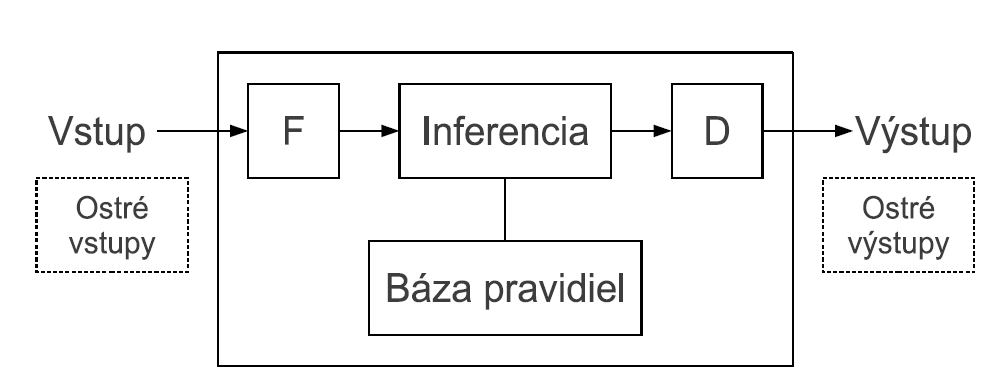
\includegraphics[width=0.75\textwidth]{obrazky/obrazok1}
	\centering
	\caption{Fuzzy inferenčný systém - bloková schéma.\cite{gregorUI}}
	\label{fig:fis}
\end{figure}

\subsubsection{Báza pravidiel}
Fuzzy inferenčný systém pri odvodzovaní nových faktorov vychádza z určitých vopred daných pravidiel. Tie sú združené v báze pravidiel. Pravidlá majú vo všeobecnosti nasledujúci tvar \cite{gregorUI, gregorRef19, gregorref1}
%tuto cituje 19 zdroj
\begin{quote}\centering
         \textbf{AK} (predpoklad)   \textbf{POTOM} (dôsledok), resp. \\
         \textbf{IF} (antecedent)  \textbf{THEN} (consequent).
\end{quote}
Predpoklad sa pritom skladá z termov nasledujúceho tvaru \cite{gregorUI}
\begin{equation}\label{baza1}
X \hspace{0.2cm} is \hspace{0.2cm}  A_i , 
\end{equation}
kde X je lingvistická premenná a $A_i$ je i-tá lingvistická hodnota tejto premennej. 

% 28-29 strana
\subsubsection{Fuzzifikácia}
Z blokovej schémy na Obr. \ref{fig:fis} je zrejmé, že do fuzzy inferenčného systému môžu vstupovať ostré hodnoty. Aby bolo možné vykonať porovnanie podľa (\ref{baza1}), ostrú vstupnú hodnotu je potrebné previesť na fuzzy množinu. Tento proces sa nazýva fuzzifikácia. Fuzzifikácia je prevod ostrej hodnoty x na fuzzy množinu $L_x$, pričom výstupom je často singleton \cite{gregorUI}
\begin{equation}\label{fuzzysingle1}
L_x = \left\lbrace1/x\right\rbrace .  
\end{equation}
Majme term v tvare podľa (\ref{baza1}). Ak ostrá hodnota premennej je x a jej fuzzifikovaná hodnota  $L_x$, potom takýto term možno vyhodnotiť jednoducho pomocou zvolenej T-normy (analógia prieniku). Ako T-norma sa v tomto prípade spravidla používa operátor minima  $T_m(a, b)=min(a, b)$. Ak sa aplikuje na dané operandy vznikne \cite{gregorUI}
\begin{equation}\label{fuzzimin}
\alpha_x = min(L_x, A^{i}) \forall x \in U, 
\end{equation}
kde $\alpha_x$ možno považovať za mieru platnosti tvrdenia (\ref{baza1}). 
Vzhľadom na vlastnosti singletonov možno tento postup zjednodušiť na 
\begin{equation}\label{fuzziminsingle}
\alpha_x = \left\lbrace \mu_{A^i}(x)/x\right\rbrace , 
\end{equation}
Keďže $\alpha_x$ je tiež singleton, tak stačí, ak sa vyjadrí iba ako $\mu_{A^i}(x)$, čo je ostré číslo. 
Fuzzifikácia v praxi je vyhodnotenie miery platnosti predpokladu X is A (\ref{baza1}) na základe znalosti ostrej hodnoty x premennej X. Miera platnosti takého predpokladu je pritom ekvivalentná stupňu príslušnosti ostrej hodnoty x ku fuzzy množine A, čiže  $\mu_{A}(x)$. \cite{gregorUI}  

%treba definovať T=normu?????? 
\pagebreak








\pagebreak
\section{Transformácia číselných hodnôt na lingvistické premenné}





















\pagebreak
\section{Meranie Entropie}
Entropia je meraná množstvom neistoty výsledku náhodného experimentu, alebo equivalene, meraním informácií keď sa pozoruje výsledok. Tento koncept bol zadefinovaný rôznymi spôsobmi [25]–[30] a zovšeobecnený v rozličných aplikovaných oblastiach, ako napríklad teória komunikácie, matematiky, štatistickej termodynamike a ekonómii [31]–[33]. Z pomedzi týchto rozličných definícií, Shannon prispel k najširšej a najfundamentálnejšej definícii entropie v informačnej teórii. V nasledujúcom texte najprv uvedieme Shannonovu entropiu a potom popíšeme štyry Luca-Termini axiómy [25], ktoré dobre-definovaná entropia musí spĺňať. Nakoniec navrhneme meranie fuzzy entropie, ktoré je rozšírenie Shannonovej definície.

\subsection{Shannonova Entropia}
Za entropiu možno považovať meranie neistoty náhodnej premennej X. Nech X je náhodná spočítateľná premenná s konečnou N-znakovou abecedou danou   .
Ak výsledok $x_j$ sa vyskytuje s pravdepodobnosťou p($x_j)$, tak potom množstvo informácie spojené so známim výskytom výstupu $x_j$ je definované ako:

1. TODO
To znamená, že pre diskrétne zdroje, informácie získané výberom symbolu sú bitové. V priemere, symbol  bude vybratý -krát z celkového počtu N výberov, takže priemerné množstvo informácie získanej z nzdrojových výsledkou je:

2. TODO 

\begin{equation}\label{fuzzy}
D_j = \frac{ \sum\limits_{r \in S_{C_{j}}(r_n)  } \: \mu_{\tilde{A}} (r) }{\sum\limits_{r \in X  } \mu_{\tilde{A}} (r) }
\end{equation}




Podelením (2.) číslom n získame priemerné množstvo informácie na symbol výstubu zdroja. To je známe ako priemerná informácia, neistota, alebo entropia definovaná nasledovne.
Definícia 1:  Entropia H(X) náhodnej diskrétnej premennej X je definovaná ako 

3. TODO
Alebo
4.	TODO
Kde
Všimnite si, že entropia je funkcia distribúcie X. Nezáleží na skutočných hodnotách náhodnej premennej X, ale iba na pravdepodobnostiach. Preto entropiu možno zasísať ako H(p).


\section{TODO INE }

\section{Záver}
\chapter{Analýza existujúcich algoritmov pre fuzzifikáciu numerických hodnôt} 

\section{Fuzzy klasifikátor s možnosťou výberu na základe fuzzy entropie }

Táto kapitola popisuje efektívny fuzzy klasifikátor s možnosťou výberu založenom na meraní fuzzy entropie (FEBFC).
Fuzzy entropia je použitá na vyhodnotenie informácie o distribúcii vzorov v priestore vzorov. S touto informáciou vedia rozdeliť priestor vzorov na disjunktné rozhodovacie regióny pre rozoznávanie vzorov. Vďaka tomu, že rozhodovacie regióny sú disjunktné, aj komplexnosť, aj výpočtová náročnosť je zredukovaná, a tým pádom aj čas trénovania a klasifikácie je extrémne krátka. Hoci rozhodovacie regióny sú rozdelené do disjunktných pod priestorov, môžu dosiahnuť kvalitnú klasifikáciu vďaka tomu, že pod priestory boli správne stanovené navrhovaným meraním fuzzy entropie. Okrem toho môžem skúmať ďalšie využitie fuzzy entropie na vybraté prvky. Procedúra výberu prvkov nielenže znižuje dimenziu problému, ale aj redukuje šum, zbytočné a nedôležité prvky. 
\subsection{Opis upravenej fuzzy entropie}

todo - word
\subsection{Algoritmus FEBFC}
Algorimus FEBFC sa skladá z nasledujúcich krokoch: 
\begin{description}
	\item[Krok 1.] Zistenie počtu intervalov pre každú dimenziu. 
	\item[Krok 2.] Zistenie centra a šírku pre každý interval.
	\item[Krok 3.] Priradenie funkcie príslúšnosti pre každý interval. 
	\item[Krok 4.] Označenie tried pre každý rozhodovací región.   

\end{description}

\section{Minimum description length partition}	

1. MDLP method developed in the
Fayyad, U. M. and Irani, K. B. (1993). Multi-interval discretization of continuous-valued attributes for classification learning, Artificial intelligence, 13, 1022-1027.
I had an interactive version of the program, which lets you choose from several stopping criteria:
1) using the criteria proposed in the original work;
2) criteria for the number of partitions intevalov;
3) criteria for the threshold Gini index (which assesses the effectiveness of the partition at the point in terms of the decrease in entropy).

\subsection{Algoritmus MDLP}

\section{Záver}	
\chapter{Implementácia algoritmov pre fuzzifikáciu numerických hodnôt} 

\section{Implementácia Algoritmu FEBFC}

\section{Modifikácia Algoritmu FEBFC}

\section{TODO = DRUHY algoritmus}

\section{TODO INE }

\section{Záver}	
\chapter{Experimentálny výskum} 

V tejto kapitole opisujem experimentálne porovnanie algoritmov na rôznych vstupných dátach. 

\section{Vstupné súbory}
Zdroje dát boli na realizáciu experimentálneho výskumu boli použité dáta z UMCI Machine Learning Repository \cite{bache2013}. 
Tieto dáta sú využívané na experimentálne porovnania metód a algoritmov získania znalostí.
Pre realizáciu experimentov boli použité súbory, ktorých výstupný atribút nadobúda hodnoty z konečnej množiny celočíselných hodnôt. 

V experimentov som použila nasledovné súbory, ktorých súbor dát obsahuje: 
\begin{itemize}
	\item \textbf{Iris}  - výsledky merania parametrov kvetov kosatcov. Výstupný atribút je typ jedného z troch druhov kvetov.  
	\item \textbf{Heart} - výsledky merania  rôznych ukazovateľov pacientov, trpiacich na srdcovo-cievne ochorenie. Výsledný atribút opisuje stupeň vážnosti ochorenia. 
	\item \textbf{Seeds} - dáta získané ako výsledok merania geometrických vlastností zŕn troch rozličných odrôd pšenice v Inštitúte geofyziky Poľskej akadémie vied. 
	
	\item \textbf{Wine} - dáta chemických ukazovateľov rôznych druhov juhotalianských vín. Vstupné atribúty obsahujú ingrediencie vo víne. Výstupný atribút určuje jeden z troch druhov vína. 
	
	\item \textbf{Yeast} - slúži na predikciu umiestnenia proteínov v bunkách kvasiniek. 

\end{itemize}


Základné charakteristiky vybraných súborov sú: 

\begin{itemize}
 \item počet pozorovaní, 
 \item počet vstupných atribútov, nadobúdajúcich lingvistické alebo číselné hodnoty, 
 \item počet variantov výstupného atribútu, 
 \item hodnota počiatočnej chyby výberu. 
\end{itemize}


V tabuľke č. \ref{table:suborydat} sú hodnoty charakteristík vybraných súborov dát.


\begin{table}[h!]
	\centering
\begin{tabular}{|p{1,4cm}|p{2cm}|p{2cm}|p{2,35cm}|p{2cm}|p{2,2cm}|p{2cm}|}
	\hline 
	
	Súbor dát & Počet  \mbox{pozorovaní} & Počet \mbox{výstupných} atribútov&
   Počet \mbox{lingvistických} atribútov&
    Počet \mbox{číselných} atribútov& 	
	P. variantov výstupného atribútov  & \mbox{Počiatočná} chyba výberu \\ 
	\hline 
	
	Heart & 270 & 13 &8& 5 & 2 & 0,4444 \\ 
	\hline 
	Iris & 150 & 4 &0 &4& 3 & 0,6667 \\ 
	\hline 
	Seeds & 210 & 7&0 & 7 & 3 & 0,3490 \\ 
	\hline 
	Wine & 178 & 13&0&13& 3 & 0,6011 \\ 
	\hline 
	Yeast & 1484 & 8 &2& 6 & 10 & 0,6880 \\ 
	\hline 	
\end{tabular} 
	\caption{Hodnoty charakteristík vybraných súborov dát.}
\label{table:suborydat}
\end{table}


\section{Súbor údajov Iris}

\subsection{Opis vstupných dát}
Je to najznámejšia databáza, ktorá sa nachádza v literatúre rozpoznávania vzorov. Súbor údajov obsahuje 3 triedy po 50 prípadoch, kde každá trieda sa vzťahuje na typ rastliny dúhovky. Jedna trieda je lineárne oddeliteľná od ostatných 2; Tieto nie sú lineárne oddeliteľné od seba. 
%todo citovat Https://archive.ics.uci.edu/ml/datasets/Iris

Prvé atribút je dĺžka sepálu v cm, druhý atribút je šírka sepálu v cm, tretí atribút dĺžka okvetných lístkov v cm, štvrtý atribút je šírka okvetných lístkov v cm. Výstupný atribút má triedy - Iris Setosa, Iris Versicolour, Iris Virginica. 

\begin{table}[h!]
\centering

\label{suhrne-statistiky-iris}
\begin{tabular}{|l|l|l|l|l|l|}
\hline
\textbf{Atribút} & \textbf{Min} & \textbf{Max} & \textbf{Mean} & \textbf{SD} & \textbf{Korelácia} \\ \hline
Dĺžka sepálu & 4,3 & 7,9 & 5,84 & 0,83 & 0,7826 \\ \hline
Šírka sepálu & 2,0 & 4,4 & 3,05 & 0,43 & -0,4194 \\ \hline
Dĺžka okvetného lístka & 1,0 & 6.9 & 3.76 & 1.76 & 0.9490 \\ \hline
Šírka okvetného lístka & 0.1 & 2.5 & 1.20 & 0.76 & 0.9565 \\ \hline
\end{tabular}
\caption{Súhrnné štatistiky pre databázu Iris}
\end{table}
\subsection{Výsledky fuzzifikácie}

Výsledky fuzzifikácie sú v tabuľke č.\ref{vysledky-tabulka-iris}. V tabuľke som vybrala som hodnotu entropiu pre atribút prvý a umiestnenie centier pre atribút štvrtý.  
\begin{table}[]
\centering
\label{vysledky-tabulka-iris}
\begin{tabular}{|l|c|c|l|}
\hline
\textbf{} & \textbf{Počet intervalov} & \textbf{\begin{tabular}[c]{@{}c@{}}Hodnota entropie \\ pre atribút 1\end{tabular}} & \multicolumn{1}{c|}{\textbf{\begin{tabular}[c]{@{}c@{}}Umiestnenie \\ centier pre atribút 4\end{tabular}}} \\ \hline
\textbf{Algoritmus 1} & 2,2,3,3,3 & 4,4680315 & 0,0600  0,5154   0,8225 \\ \hline
\textbf{Algoritmus 2} & 2,2,5,3,3 & 2,2678531 & 0,0600 0,5154  0,8225 \\ \hline
\textbf{Algoritmus 3} & 3,3,4,4,3 & 6,8543783 & 0,0600  0,4722  0,6595  0,8822 \\ \hline
\textbf{Algoritmus 4} & 5,2,3,4,3 & 1,6914607 & 0,0000  0,0417 0,3750  0,4583 \\ \hline
\end{tabular}
\caption{Výsledky fuzzifikácie Iris databázy.}

\end{table}

\subsection{Experiment - Vývoj hodnoty entropie }
Experiment spočíva v sledovaní vývoja hodnoty entropie prvého atribútu v  intervale $<2,22>$. Hodnota entropie pri Algoritme 1 stúpa, zatiaľ čo algoritmy čo používajú váženú entropiu, sa hodnoto udržujú na rovnakej úrovni.  Počet tried na intervale tri je priemerne pre triedy 60, 60, 30. 
\begin{figure}[ht!]
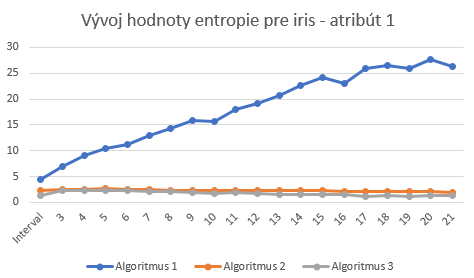
\includegraphics[width=0.75\textwidth]{obrazky/iris-vyvoj-entropie-atribut1.PNG}
\centering
\caption{Vývoj hodnoty entropie pre iris - atribút 1. } 
\label{fig:structure}
\end{figure}

\section{Súbor údajov vína}

\subsection{Opis vstupných dát}
Tieto údaje sú výsledkom chemickej analýzy vín pestovaných v rovnakom regióne v Taliansku, ale odvodených od troch rôznych kultivarov. Analýza určila množstvo 13 zložiek, ktoré sa nachádzajú v každom z troch druhov vín. 
%https://archive.ics.uci.edu/ml/datasets/Wine

 Počet inštancií je 178, z toho v triedach je 59, 71, 48 položiek.  Prvý atribút je identifikátor triedy. Počet atribútov má 4 číselných, 1 prediktívný atribút a triedu. 
Názvy atribútov: Alkohol , Kyselina jablčná, Popol 
, Alkalinity popola 
, Horčík 
, Celkové fenoly 
, Flavanoidy
, Neflavanoidné fenoly
, Proantokyaníny 
, Intenzita farieb
, Odtieň 
, OD280 / OD315 zriedených vín 
, Prolín. 



\subsection{Výsledky fuzzifikácie a experimenty}
Výsledky fuzzifikácie sú v tabuľke č.\ref{vysledky-tabulka-wine}. Počet tried pre atribút prvý je 61, 56, 61. 
Experiment spočíva v sledovaní vývoja hodnoty entropie prvého atribútu. 

\begin{table}[]
\centering

\label{vysledky-tabulka-wine}
\begin{tabular}{|l|c|l|l|}
\hline
\textbf{} & \textbf{\begin{tabular}[c]{@{}c@{}}Hodnota entropie \\ pre atribút 1\end{tabular}} & \textbf{\begin{tabular}[c]{@{}l@{}}Hodnota entropie \\ pre atribút 1  ($I+1$) \end{tabular}} & \multicolumn{1}{c|}{\textbf{\begin{tabular}[c]{@{}c@{}}Umiestnenie centier\\ pre atribút 1\end{tabular}}} \\ \hline
\textbf{Algoritmus 1} & 4,8846493 & 7,6232103 & 0,3289  0,6919 \\ \hline
\textbf{Algoritmus 2} & 2,7733194 & 2,8339819 & 0,3289 0,6919 \\ \hline
\textbf{Algoritmus 3} & 4,8846493 & 7,6232103 & 0,2779 0,5232 0,7550 \\ \hline
\textbf{Algoritmus 4} & 1,1502002 & 2,1532059 & 0,1395 0,1553 \\ \hline
\end{tabular}
\caption{Výsledky fuzzifikácie Wine databázy.}
\end{table}

\begin{figure}[ht!]
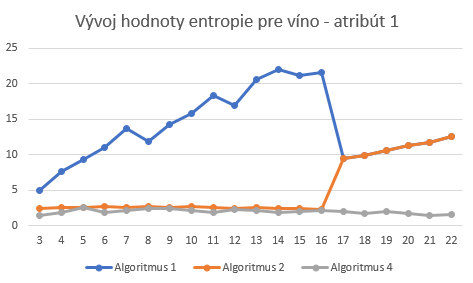
\includegraphics[width=0.75\textwidth]{obrazky/wine-vyvoj-entropie-atribut1.PNG}
\centering
\caption{Vývoj hodnoty entropie pre víno - atribút 1} 
\label{fig:structure}
\end{figure}

\section{Súbor údajov kvasníc (Yeast)}
%https://archive.ics.uci.edu/ml/datasets/Yeast
Údaje sú na predpovedanie bunkovej lokalizácie proteínov. 
Počet inštancií je  1484 pre súbor údajov o kvasinkách.
 Počet atribútov pre súbor kvasiniek je 9 (8 prediktívnych, 1 názov): 
\begin{enumerate}
\item Názov série: Prístupové číslo pre databázu SWISS-PROT
\item mcg: McGeochova metóda na rozpoznávanie signálových sekvencií.
\item gvh: von Heijneov metóda pre rozpoznávanie signálnej sekvencie.
\item alm: Skóre prognózového programu ALOM membránovej oblasti.
\item mit: Skóre analýzy obsahu aminokyselín.
\item erl: Prítomnosť substringu "HDEL". Binárny atribút.
\item pox: Peroxizomálny cieľový signál na C-konci.
\item vac: Skóre rozlišovacej analýzy obsahu aminokyselín v
Vakuolárne a extracelulárne proteíny.
\item nuc: Skóre analýzy jadrových lokalizačných signálov.

\end{enumerate}
 Distribúcia tried je nasledovná : 
\begin{itemize}
\item CYT (cytosolický alebo cytoskeletálny) - 463
\item NUC (nukleárne)  - 429
\item MIT (mitochondriálna)  - 244
\item ME3 (membránový proteín, žiadny N-koncový signál) -  163
\item ME2 (membránový proteín, neštiepený signál)  - 51
\item ME1 (membránový proteín, štiepený signál)  - 44
\item EXC (extracelulárne)  - 37
\item VAC (vakuolárne)  - 30
\item POX (peroxisomálny) - 20
\item ERL (endoplazmatický retikulový lumen) -  5
\end{itemize}
Výsledky fuzzifikácie sú v tabuľke č. \ref{my-label44}
\begin{table}[hp!]
\centering
\begin{tabular}{|l|c|l|l|}
\hline
\textbf{} & \textbf{\begin{tabular}[c]{@{}c@{}}Hodnota entropie \\ pre atribút 1\end{tabular}} & \textbf{\begin{tabular}[c]{@{}l@{}}Hodnota entropie \\ pre atribút 1 - I+1\end{tabular}} & \multicolumn{1}{c|}{\textbf{\begin{tabular}[c]{@{}c@{}}Umiestnenie centier\\ pre atribút 1\end{tabular}}} \\ \hline
\textbf{Algoritmus 1} & 4,8846493482439 & 7,6232103794469 & 0,3289  0,6919 \\ \hline
\textbf{Algoritmus 2} & 2,77331942036114 & 2,83398191261714 & 0,3289 0,6919 \\ \hline
\textbf{Algoritmus 3} & 4,8846493482439 & 7,6232103794469 & 0,2779 0,5232 0,7550 \\ \hline
\textbf{Algoritmus 4} & 1,15020020568059 & 2,15320594479199 & 0,1395 0,1553 \\ \hline
\end{tabular}
\caption{Výsledky fuzzifikácie pre súbor dát kvasníc}
\label{my-label44}
\end{table}

\section{Súbor údajov Statlog (srdce)}
%Https://archive.ics.uci.edu/ml/datasets/Statlog+%28Heart%29
Táto sada dát je databáza srdcových ochorení. Počet inštancií je 270 a atribútov je 13.  Predpokladaná premenná je absencia (1) alebo prítomnosť (2) ochorenia srdca.
Typy atribútov:
\begin{itemize}
\item Numerické: 1,4,5,8,10,12. 
\item Usporiadané: 11. 
\item Binárne: 2,6,9. 
\item Nominálna hodnota: 7,3,13.
\end{itemize}
V tabuľke č. \ref{my-label45} sú výsledky fuzzifikácie dát. 

\begin{table}[hp!]
\centering
\begin{tabular}{|l|c|l|l|}
\hline
\textbf{} & \textbf{\begin{tabular}[c]{@{}c@{}}Hodnota entropie \\ pre atribút 1\end{tabular}} & \textbf{\begin{tabular}[c]{@{}l@{}}Hodnota entropie \\ pre atribút 1 - I+1\end{tabular}} & \multicolumn{1}{c|}{\textbf{\begin{tabular}[c]{@{}c@{}}Umiestnenie centier\\ pre atribút 1\end{tabular}}} \\ \hline
\textbf{Algoritmus 1} & 4,8846493482439 & 7,6232103794469 & 0,3289  0,6919 \\ \hline
\textbf{Algoritmus 2} & 2,77331942036114 & 2,83398191261714 & 0,3289 0,6919 \\ \hline
\textbf{Algoritmus 3} & 4,8846493482439 & 7,6232103794469 & 0,2779 0,5232 0,7550 \\ \hline
\textbf{Algoritmus 4} & 1,15020020568059 & 2,15320594479199 & 0,1395 0,1553 \\ \hline
\end{tabular}
\caption{Výsledky fuzzifikácie pre súbor dát srdce}
\label{my-label45}
\end{table}

\section{Súbor dát semien}
%https://archive.ics.uci.edu/ml/datasets/seeds
 Súbor dát je z merania geometrických vlastností jadier, ktoré patria do troch rôznych odrôd pšenice. Mäkká röntgenová technika a balík GRAINS boli použité na zostavenie všetkých siedmich atribútov s reálnou hodnotou.
 
 Informácie o atribútoch: Na zostrojenie údajov sa meralo sedem geometrických parametrov pšeničných jadier: 
oblasť A, 
obvod P, 
kompaktnosť C = $4 * pi * A / P ^ 2$, 
 dĺžka jadra, 
 šírka jadra, 
 koeficient asymetrie, 
dĺžka drážky jadra. 

V nasledujúcej tabuľke \ref{my-label33} sú výsledky pre súbor dát semien. 

\begin{table}[hp!]
\centering
\begin{tabular}{|l|c|l|l|}
\hline
\textbf{} & \textbf{\begin{tabular}[c]{@{}c@{}}Hodnota entropie \\ pre atribút 1\end{tabular}} & \textbf{\begin{tabular}[c]{@{}l@{}}Hodnota entropie \\ pre atribút 1\end{tabular}} & \multicolumn{1}{c|}{\textbf{\begin{tabular}[c]{@{}c@{}}Umiestnenie centier\\ pre atribút 1\end{tabular}}} \\ \hline
\textbf{Algoritmus 1} & 4,8846493482439 & 7,6232103794469 & 0,3289  0,6919 \\ \hline
\textbf{Algoritmus 2} & 2,77331942036114 & 2,83398191261714 & 0,3289 0,6919 \\ \hline
\textbf{Algoritmus 3} & 4,8846493482439 & 7,6232103794469 & 0,2779 0,5232 0,7550 \\ \hline
\textbf{Algoritmus 4} & 1,15020020568059 & 2,15320594479199 & 0,1395 0,1553 \\ \hline
\end{tabular}
\caption{Výsledky fuzzifikácie pre súbor dát - Semená}
\label{my-label33}
\end{table}

\section{Zhrnutie výsledkov }
Algoritmus 4 efektívne zoradí centra. Pri Algoritme 1 hodnota entropie stúpa smerom nahor. Algoritmus 2 pomocou váženej entropie je dobrý na určenie počtu intervalov, ak triedy majú nerovnomerne rozdelené prvky. Algoritmus 3 dáva vyšší počet intervalov kvôli tomu, že prahová hodnota bola nastavená nízko. 



%\section{Parametre, určujúce kvalitu fuzzifikácie}
%
%\section{Priebeh experimetnov - použité dátové množiny}
%
%\section{Výsledky a vyhodnotenie experimentov pre vybraté dátové množiny}
%
%\section{Zhrnutie výsledkov }
%
%\section{Záver}
\chapter*{Záver}




















%%%%%%%%%%%%%%%%%%%%%%%%%%%%%%%%%%%%%%%%%%%%%%%%%%%%%%%%%%%%%%%%%%%%%%%%%%%%%
\begin{thebibliography}{}                               
	 \label{literatura}
%\bibitem{urlZdroj}\url{https://github.com/chovancova/diploma-thesis-fuzzification} 

%\bibitem{Priezvisko} Priezvisko M., {\it Názov knihy, clanku} , 
%Vydavatelstvo, 2013, ISBN 978-1-449-36536-3

\bibitem{levashenkoProj} LEVASHENKO V. - ZAITSEVA E. - KOVALÍK Š. {\it Projektovanie systémov pre podporu rozhodovania na základe neurčitých dát}. Žilinská univerzita v Žiline/EDIS, 2013. ISBN 978-80-554-0680-0.

%todo zjednotit bodky a ciarky v referenciach

\bibitem{Zadeh1965} Zadeh L., {\it Fuzzy sets}. Information and Control, vol.8, 1965, pp. 338-353. 

\bibitem{Kaufman1985} Kaufmann A., Gupta M., {\it Induction to fuzzy arithmetic: theory and applications}. New York : Van Nostrand Reinold Co., 1985, 361 p. 
\bibitem{Klir1995}
Klir G., Yuan B., {\it Fuzzy Sets and Fuzzy Logic. Theory and Applications}. Prentice Hall, 1995, 591 p. 
\bibitem{Navara2011}
Navara M., {\it Computation with fuzzy quantities}. Proc. of the 7th Conf. of the European Society for Fuzzy Logic and Technology (EUSFLAT), Aix-les-Bains, France, 2011, pp. 209-214.






\bibitem{gregorUI} GREGOR M., {\it Umelá inteligencia 1} , CEIT, 2014, ISBN 978-80-971684-1-4.
%kniha o umelej inteligencii = jeho prva referencia
\bibitem{gregorref1} SPALEK.J - JANOTA. A - BLAŽOVIČOVÁ, M. - PŘIBYL, P. {\it Rozhodovanie a riadenie s podporou umelej inteligencie}. Žilinská univerzita v Žiline/EDIS, 2005. ISBN 80-8070-354-X. 

\bibitem{gregorRef13} NICKLES. M - SOTTARA, D. {\it Approaches to Uncertain or Imprecise Rules - A Survey}. In Rule Interchange and Applications, vol. 5858 of {\it Lecture Notes in Computer Science}, pp. 323-336. Springer, 2009. ISBN 9783642049842. 

%pozri a najdi tento zdroj - Ross, T.J. Fuzzy Logic with Engineering Applications. .. alebo pozri zdroje v knihe 14
\bibitem{gregorRef14} ROSS, T.J. {\it  Fuzzy Logic with Engineering Applications.}. John Wiley \& Sons, 2004, second edition ed. ISBN 0-470-86075-8. 



\bibitem{gregorRef19}PASISNO, K. M. - YURKOVICH, S. {\it Fuzzy control}, vol.42. Addison Wesley Longman, 1998. ISBN 0-201-18074-X.  


\bibitem{Garcia2013} García S., Luengo J. Sáes J.A., López V., Herrera F., \textit{ A Survey of Discretization Techniques: 	Taxonomy and Empirical Analysis	in Supervised Learning }
IEEE TRANSACTIONS ON KNOWLEDGE AND DATA ENGINEERING, VOL. 25, NO. 4, 2013, pp. 734-750.




%Wong1987
\bibitem{Wong1987} 
Wong A.K., Chiu D.K., {\it Synthesizing Statical Knowledge from Incomplete Mixed-Mode Data}. IEE Trans. on Pattern Analysiss and Machine Intelligence, vol.9, no.6, 1987, pp. 796-805. 

%Keber1992
\bibitem{Keber1992} 
Kerber R., {\it ChiMerge: Discretitation of numeric attributes}. Proc. of the 9th National Conf. on Artifical Intelligence American Association for Artifical Intelligence, 1992, pp.123-128. 

%Quinlan1993
\bibitem{Quinlan1993} 
Quinlan J.R, {\it C4.5: Programs for Machine Learning}. Morgan Kaufmann Publ. Inc, San Manteo, California, 1993. 


%Fayyad1993
\bibitem{Fayyad1993} 
Fayyad U.M., Irani K.B., {\it Multi-Interval Discretitation of Continuous-Valued Attributes for Classification Learning}, 
Proc. of the 13th Int. Joint Conf. on Artifical Intelligence, 1993, pp. 1022-1027. 


%Ventura1994
\bibitem{Ventura1994} 
Ventura D., Martinez T. R., {\it BRACE: A paradigm for the discretization of Continuously valued data. } 
Proc. of the 7th Annual Florida AI Research Symposium (FLAIRS), 1994, pp. 117-121. 


%Pazzani1995
\bibitem{Pazzani1995} 
Pazzani M.J., {\it An iterative improvement approach for the discretization of numeric attributes in bayesian classifiers}.
Proc. of the Int. Conf. on Knowledge Discovery and Data Mining (KDD), 1995, pp. 228-233. 


%Ching1995
\bibitem{Ching1995} 
Ching J.Y., Wong A.K.C., Chan, K.C.C., {\it Class-Dependent Diskretization for Inductive Learning from Continuous and Mixed-Mode Data}.
IEEE Trans. on Pattern Analysis and Machine Intelligence, vol.17, no.7, 1995, pp. 641-651.


%Liu1997
\bibitem{Liu1997} 
, {\it  }


%Ho1997
\bibitem{Ho1997} 
, {\it  }


%Monti1998
\bibitem{Monti1998} 
, {\it  }


%Grzymala2001
\bibitem{Grzymala2001} 
, {\it  }


%Bay2001
\bibitem{Bay2001} 
, {\it  }


%Giraldez2002
\bibitem{Giraldez2002} 
, {\it  }


%Kurgan2004
\bibitem{Kurgan2004} 
, {\it  }


%Chao2005
\bibitem{Chao2005} 
, {\it  }


%Mehta2005
\bibitem{Mehta2005} 
, {\it  }


%Ferrandiz2005
\bibitem{Ferrandiz2005} 
, {\it  }


%Boulle2006
\bibitem{Boulle2006} 
, {\it  }


%Au2006
\bibitem{Au2006} 
, {\it  }


%Lee2007
\bibitem{Lee2007} 
, {\it  }


%Flores2007
\bibitem{Flores2007} 
, {\it  }


%Ruiz2008
\bibitem{Ruiz2008} 
, {\it  }


%Hu2008
\bibitem{Hu2008} 
, {\it  }


%Berrado2009
\bibitem{Berrado2009} 
, {\it  }


%Jiang2009
\bibitem{Jiang2009} 
, {\it  }


%Jin2009 - založený na pojmoch teórie informácie. 
\bibitem{Jin2009} 
, {\it  }


%Yang2009a
\bibitem{Yang2009a} 
, {\it  }


%Jiang2009
\bibitem{Jiang2009} 
, {\it  }


%Nemmiche2010
\bibitem{Nemmiche2010} 
, {\it  }


%Zhu2010
\bibitem{Zhu2010} 
, {\it  }


%Li2010a
\bibitem{Li2010a} 
, {\it  }


%Gupta2010
\bibitem{Gupta2010} 
, {\it  }


%Sang2010
\bibitem{Sang2010} 
, {\it  }


%Garcia2010
\bibitem{Garcia2010} 
, {\it  }



        
\end{thebibliography}

	%  Literatura
%%%%% \MakeBibliography 

\appendix
%\chapter{UML diagramy}
\section*{Diagram tried nástroja Fuzzy Tool}
\begin{figure}[h]
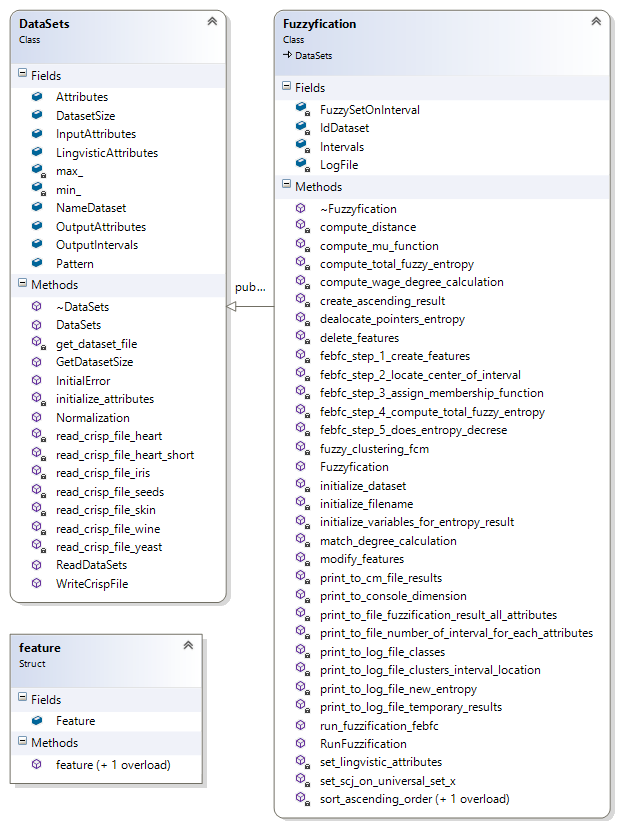
\includegraphics[width=1\textwidth]{obrazky/ClassDiagram2.png}
\centering
\caption{Diagram tried nástroja Fuzzy Tool} 
\label{fig:diagramTried}
\end{figure}

\end{document}